\chapter{Fourth Species of Counterpoint}

The fourth species of counterpoint consists of syncopations\footnote{Syncopation creates an off-balance rhythm through the accenting of normally unaccented beats.}, one note\footnote{Or rather two half notes with the same pitch.} shifted half a measure late against one note. In other words, only pairs of half notes\footnote{Except that the penultimate measure never has syncopation and it happens in certain measures that no syncopation is available.}.
\begin{figure}[h]
    \centering
    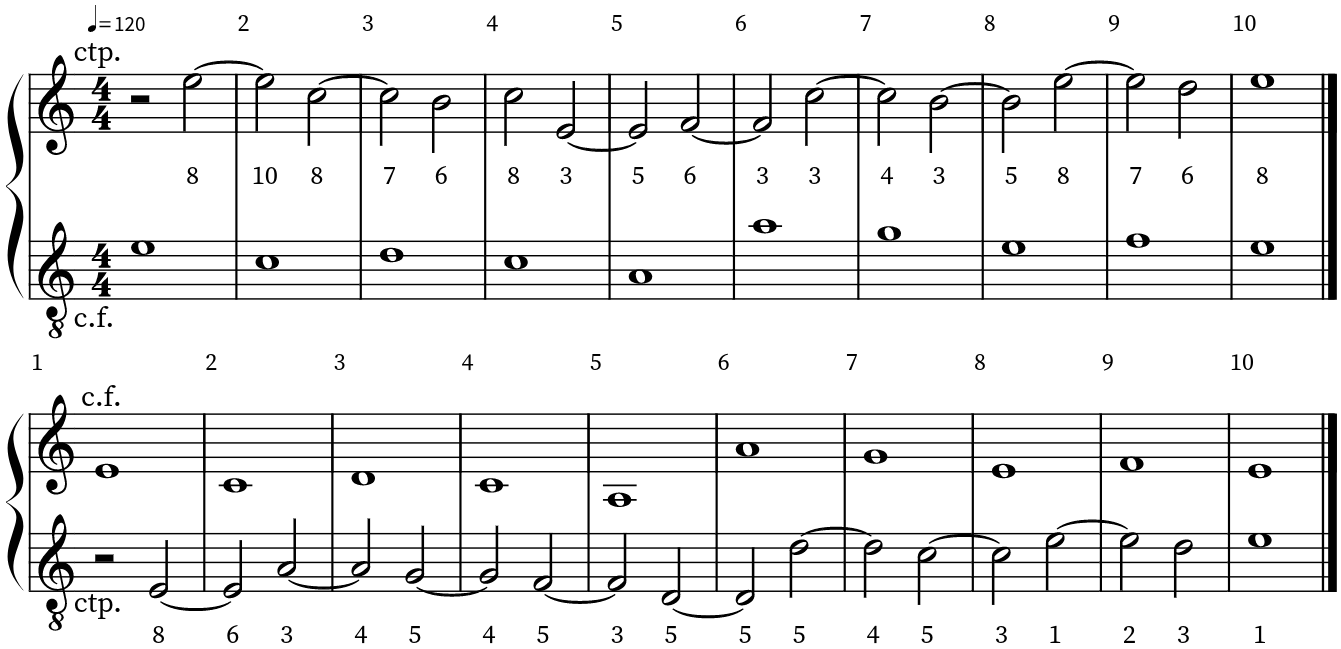
\includegraphics[width=5in]{Images/the_fourth_species.png}
    \caption{Two \species{4} ctp. \listen{Listen4SP} \listenyt{https://youtu.be/9yB4OGr4Cgk?t=184}}
\end{figure}

The fourth species is particular because it does not have more notes than the preceding species, it even has less. Indeed, this species is more like the first one. Here the syncopations are delays, which is roughly equivalent to using the first species with the whole note in thesis shifted in arsis which then lasts until the next arsis beat. While in the first species, all notes were consonant, here the syncopation requires more flexibility because the same whole note (here represented by a pair of half notes) is confronted with two different notes of the \cfdot First the second half of the first and then the first half of the second. If the syncopation is a delay of the note in thesis, then it is logical that the harmony it creates in arsis must be consonant (see rule \ref{rule:arsiscons}). The specificity of the fourth species comes from the fact that dissonances can appear in thesis.

\section{Formalization in English}
For a better reading experience, the subsection on motion rules has been placed first as it is fundamental to understanding the other types of rules.

\subsection{Motion Rules of the Fourth Species}
For this species, no rule concerning the motions is given by Fux. Moreover, no invariant, which could have served as a basis for creating an implicit rule, has been found in these examples. From another point of view, it could be seen that the motion created by a syncopation is nothing else than the oblique motion because one note stays in place while the other changes. This is of little importance because the rules concerning motions are somewhat adapted by rule \ref{rule:nosecond}.
\begin{enumerate}[wide, label=\bfseries 4.P\arabic*]
    \item\label{rule:dissolved} \textit{Dissonant harmonies must be followed by the next lower consonant harmony.} \textcite[p.78-81]{GaPFr}

    Any dissonant syncopation\footnote{A dissonant syncopation is a syncopation that becomes dissonant at the changing note of the \cfdot It differs from a consonant syncopation which is strictly always consonant with the \cfdot} should be resolved by moving downwards. This implies that if the \cf is below, a second will resolve into a unison, narrowing the harmonic gap. Whereas if the \cf is above, a second will resolve into a third, widening the harmonic gap. Figure \ref{fig:dissonantdown} shows some examples of this rule.

    \begin{figure}[h]
        \centering
        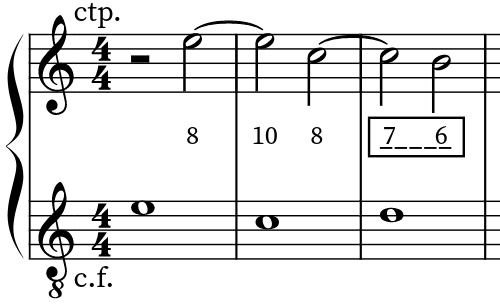
\includegraphics[height=\fh]{Images/dissonance_resolved.png}
        \caption{Dissonant syncopations resolved, \species{4}.}
        \label{fig:dissonantdown}
    \end{figure}

    \item\label{rule:nosecond} \textit{If the \cf is in the lower part then no second harmony can be preceded by a unison/octave harmony.} \parencite[p.79-80]{GaPFr}

    The idea behind this rule is that \emph{no octave/unison harmony in arsis can be followed by an octave/unison harmony in the next arsis with a dissonant harmony in between}. It is a kind of adaptation of rule \ref{rule:nopconsbydm} which says that perfect consonances cannot be reached by direct motion. Indeed, according to rule \ref{rule:dissolved}, a second that is dissonant must resolve into a unison. This would result in a unison sequence (see figure \ref{fig:secondpreuni}) if the retardation is removed, i.e. the second, which would violate rule \ref{rule:nopconsbydm}.
    \begin{figure}[h]
        \centering
        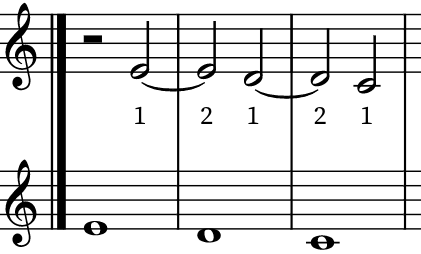
\includegraphics[height=\fhs]{Images/unisons_succ.png}
        \caption{Seconds preceded by a unison, \species{4}.}
        \label{fig:secondpreuni}
    \end{figure}

    Now, let's dive into the in-depth logic of this rule. Although Fux's explanation is logical and the rule is applied in his examples, the logic itself is not applied to other similar problems later on. An example will speak for itself:
    \begin{figure}[h]
        \centering
        \begin{subfigure}{.4\textwidth}
            \centering
            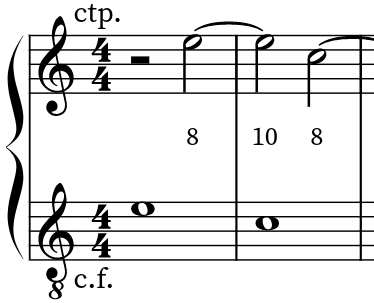
\includegraphics[height=1.1in]{Images/consecutives_octaves.png}
            \caption{Two consecutive arsis octaves.}
            \label{fig:twoarsisoctaves}
        \end{subfigure}%
        \begin{subfigure}{.6\textwidth}
            \centering
            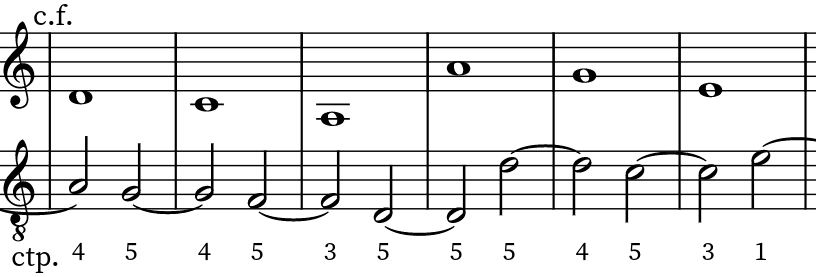
\includegraphics[height=1.1in]{Images/consecutives_fifths.png}
            \caption{Two consecutive arsis fifths.}
            \label{fig:twoarsisfifths}
        \end{subfigure}
        \caption{Consecutive perfect consonances in arsis, \species{4}.}
    \end{figure}

    In figure \ref{fig:twoarsisoctaves}, a consonant syncopation consisting of an octave and a third\footnote{Here the third is actually a tenth.} is then followed by an octave again. No problem, the rule is respected since no second has appeared, but why put an octave whereas if the delay is removed, one falls back into the same issue that originated this rule, (i.e. two consecutive arsis octaves)? \textcite[p.95]{GaPEng} suggests that "[\dots] in measures containing dissonant syncopations the essential part is the upbeat, the second, consonant, half." This can be paraphrased to say that the human ear is only interested in the first consonance of a measure. This explains why the succession of octaves in the previous figure \ref{fig:twoarsisoctaves} is not one. Because the consonant third cuts off this impression.
    
    What about fifths, which are also perfect consonances? In figure \ref{fig:twoarsisfifths}, a consonant fifth ($G-D$) turns into a dissonant fourth ($G-C$) which is, as rule \ref{rule:dissolved} requires, resolved into a fifth again ($F-C$). There is clearly a succession of fifths. But for a reason that Fux does not detail but that \textcite[p.57]{GaPEng} points out: "In the case of fifths, however, the retardation can mitigate the effect of parallel motion. Successions of fifths may therefore be used with syncopations." Probably because the fifth brings a little harmony where the octave does not really\footnote{The octave is the simplest harmonic of its basic note with a frequency ratio of 2:1. Since it is the same note in a higher register it is not really about "harmony" as such. \parencite{Octavei}}. It is therefore only the current rule \ref{rule:nosecond} specific to octaves that is admitted.

    All this thinking is explained for a reason: the purpose of the final software is to assist a composer and that he can choose thanks to an obvious logic that some rules are obsolete in his own case. It is therefore preferable to have logical rules such as "no two perfect consonances in a row without another imperfect consonance in between". This rule would be more contextual, more global and would speak more to a composer. Here, the rule is adapted only for octaves so that it keeps the associated logic instead of explaining it in the form of forbidding a second after a unison.
    
\end{enumerate}

\subsection{Harmonic Rules of the Fourth Species}

\begin{enumerate}[wide, label=\bfseries 4.H\arabic*]
    \item\label{rule:arsiscons} \textit{Arsis harmonies must be consonant.} \parencite[p.78]{GaPFr}
    
    Although explicitly described by Fux, this rule is only an adaptation of fundamental rule \ref{rule:allcons} as explained above.

    \item\label{rule:noseventh} \textit{If the \cf is in the upper part, then no harmonic seventh interval can occur.}

    The origin of this rule is the same as rule \ref{rule:nosecond}. It is just less specific and therefore more restrictive because it does not depend on the previous or next harmony. Fux explains that this rule has no logical reason to exist. Nevertheless, the authoritative composers respected it, as did Fux as a result. It is optional for the previous reason.

    \item\label{rule:lowpenult4th} \textit{For rule \ref{rule:low_penult} to be satisfied in the penultimate measure, if the \cf is in the lower part, then the harmonic interval of the thesis note must be a seventh.}

    The penultimate note cannot be a syncopation because the last note necessarily ends at the same time as the last note of the \cf (see figure \ref{fig:penultlow4sp}).
    \begin{figure}[h]
        \centering
        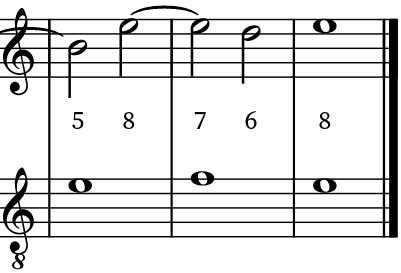
\includegraphics[height=\fh]{Images/penult_4th.png}
        \caption{Penultimate measure, \species{4}.}
        \label{fig:penultlow4sp}
    \end{figure}
    
    As usual in this case, the penultimate note is always a major sixth. The syncopation ending on the penultimate measure must be a dissonant seventh \footnote{Because of the structure of the \cfcomma the seventh is often the tonic. This is a classic melodic progression at the end of a piece in tonal music that makes I - VII - I in degree (see \textit{degree} in section \ref{sec:musictheory:terms}).}. Following rule \ref{rule:dissolved}, the dissonance is resolved to the nearest consonance below.
    
    \item\label{rule:uppenult4th} \textit{For rule \ref{rule:up_penult} to be satisfied in the penultimate measure, if the \cf is in the upper part, then the harmonic interval of the thesis note must be a second.}
    
    The logic of the previous rule also applies to this one.
\end{enumerate}

\subsection{Melodic Rules of the Fourth Species}
\begin{enumerate}[wide, label=\bfseries 4.M\arabic*]
    \item\label{rule:fullsyncopations} \textit{Arsis half notes should be the same as their next halves in thesis.}
    
    In other words, \textit{syncopations should occur if possible}. In theory, they are mandatory except in the penultimate measure. However, it happens that Fux breaks this rule to avoid monotony which is reflected by a repetition of a pattern in the musical work. This means that the cost of not putting a syncopation is lower than the cost of repeating the same syncopations. The difficulty is to know which cost best represents the monotony, which is quite subjective. Although all costs in the program have functional defaults, it's up to the composer to test various combinations to make the software shine. This will be shown in section \ref{sec:5sp_experimentation}.

    \item\label{rule:m2same} \textit{Each arsis note and its two measures further peer are preferred to be different.}

    This is a more or less implicit consequence of the previous rule and is also an adaptation of rule \ref{rule:twobeats}. For the same reason as the latter, it is better to avoid alternating only between two different syncopations. But this remains totally subjective because one could look for this very repetition in the syncopations. This is why the associated cost is customizable by the user.
\end{enumerate}

\section{Formalization into Constraints}

Note that the arrays in index $[0, 0]$ are empty because the syncope arrives two beats late and leaves a silence in first thesis.

\subsection{Motion Constraints of the Fourth Species}
\paragraph{\ref{rule:dissolved}} \textit{Dissonant harmonies must be followed by the next lower consonant harmony.}

There is no need to add the constraint $IsCons[2, j] = \top$ because it is already included by rule \ref{rule:arsiscons} (see equation \ref{eq:arsiscons}).

\begin{equation}
    \begin{gathered}
        \forall j \in [1, m-1) \quad
        \lnot IsCons[0, j] \implies M_{brut}[0, j] \in \{-1, -2\}
    \end{gathered}
\end{equation}

\begin{lstlisting}[caption=Function that constrains a dissonance to be followed by a consonance., label=lst:dissonance]
; @m-succ-intervals-brut: list of IntVar, s.f. brut melodic intervals
; @is-cons-arr: list of BoolVar, s.f. 1 -> the note is consonant
(defun add-h-dis-imp-cons-below-cst (m-succ-intervals-brut is-cons-arr)
    (loop for m in m-succ-intervals-brut for b in is-cons-arr do
    (let (
        (b-not (gil::add-bool-var *sp* 0 1)) ; s.f. !b (dissonance)
    )
        (gil::g-op *sp* b gil::BOT_EQV FALSE b-not) ; b-not = !b (dissonance)
        (gil::g-rel-reify *sp* m gil::IRT_LE 0 b-not gil::RM_IMP) ; b-not => m<0
        (gil::g-rel-reify *sp* m gil::IRT_GQ -2 b-not gil::RM_IMP) ; b-not => m>=-2
)   ))
\end{lstlisting}

\paragraph{\ref{rule:nosecond}} \textit{If the \cf is in the lower part then no second harmony can be preceded by a unison/octave harmony.}

\begin{equation}
    \begin{gathered}
        \forall j \in [1, m-1)\\
        IsCfB[j+1] \implies H[2, j] \neq 0 \land H[0, j+1] \notin \{1, 2\}
    \end{gathered}
\end{equation}

\subsection{Harmonic Constraints of the Fourth Species}
\paragraph{\ref{rule:arsiscons}} \textit{Arsis harmonies must be consonant.}

\begin{equation}
    \begin{gathered}
        \forall j \in [0, m-1) \quad
        H[2, j] \in Cons
    \end{gathered}
    \label{eq:arsiscons}
\end{equation}

\paragraph{\ref{rule:noseventh}} \textit{If the \cf is in the upper part, then no harmonic seventh interval can occur.}

\begin{equation}
    \begin{gathered}
        \forall j \in [1, m-1) \quad
        \lnot IsCfB[j] \implies H[0, j] \notin \{10, 11\}
    \end{gathered}
\end{equation}

\paragraph{\ref{rule:lowpenult4th}, \ref{rule:uppenult4th}} \textit{In the penultimate measure, the harmonic interval of the thesis note must be a major sixth or a minor third depending on the \cf pitch.}

\begin{equation}
    \begin{gathered}
        H[0, m-2] = \begin{cases}
            9 & \text{if } IsCfB[m-2]\\
            3 & \text{otherwise}
        \end{cases}
    \end{gathered}
\end{equation}

\subsection{Melodic Constraints of the Fourth Species}
\paragraph{\ref{rule:fullsyncopations}} \textit{Arsis half notes should be the same as their next halves in thesis.}

The cost of not having syncope is by default \dfts{last resort}. It is because of costs like this that it is not really possible to compare the quality of two works of the same length just with the raw cost. Indeed, some \cf may not have possibilities with syncopations only, which will artificially increase the total cost. It is therefore important to keep in mind that the costs are only relative to the \cf used.

\begin{equation}
    \begin{gathered}
        \forall j \in [0, m-1) \quad
        NoSync_{costs} = \begin{cases}
            cost_{NoSync} & \text{if } M[2, j] \neq 0\\
            0 & \text{otherwise}
        \end{cases}
    \end{gathered}
\end{equation}

\paragraph{\ref{rule:m2same}} \textit{Each arsis note and its two measures further peer are preferred to be different.}

The default cost is \dfts{high cost} because monotony is very much avoided by Fux. It is unclear whether this cost should be higher than the cost of not having syncope.

\begin{equation}
    \begin{gathered}
        \forall j \in [0, m-1)\\
        MtwomSame_{costs} = \begin{cases}
            cost_{MtwomSame} & \text{if } Cp[2, j] = Cp[2, j+2]\\
            0 & \text{otherwise}
        \end{cases}
    \end{gathered}
\end{equation}